\chapter{Player Skills}
\label{Agent}

In this chapter we are going to present the main functions that are necessary for the agent to be functional in the field. Every part of the agent's software and supported player skills will be extensively described below. 


\section{Agent Architecture}
\label{Architecture}

Before examining each individual skill of our players, it is important to describe the general architecture of our agents, which is shown in  Figure~\ref{fig:Architecture}. The Soccer Simulation Server (\textit{rcssserver3d}) is responsible for communicating perceptor messages to the agent. The Connection component handles this connection between the agent and the server. These messages are handled by a string parser, which stores the incoming observations in various data structures. Consequently, the functions that require these new observations  to update the agent's Beliefs are now ready to proceed. Self-localization of the agent into the field or a check if the agent has fallen on the ground are few of those belief updates. Behavior is a major component of any agent. The agent has to combine all the available knowledge and beliefs about the world state and act properly. Behavior is the function which takes as input argument the agent's beliefs about the world state and computes an action to be executed by the agent as output. The Coordination component is responsible for assigning roles to different agents implementing the strategy of team. Communication  and Motion are responsible for handling agent's requests for sending messages to teammates and executing movements respectively. These two components send effector messages to the Connection component in each cycle, if necessary, and these messages are relayed to the soccer simulation server.

\begin{figure}[t!]
\centering
  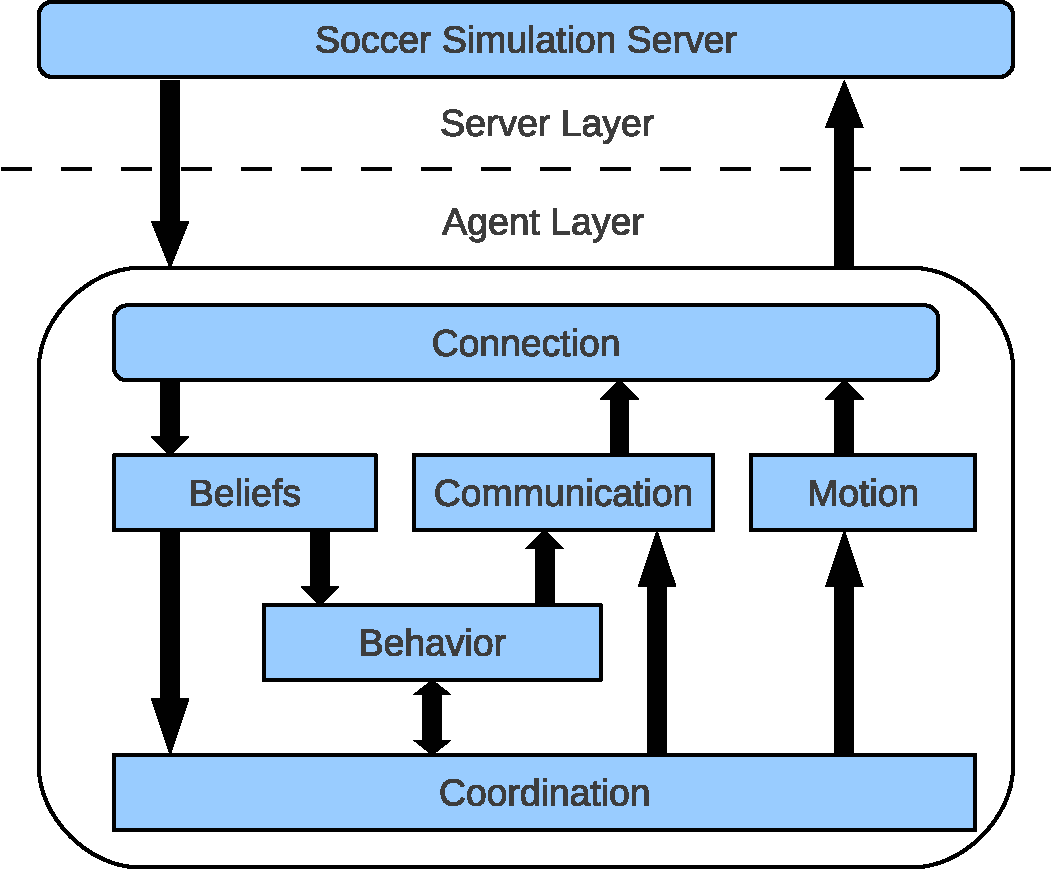
\includegraphics[width=0.8\textwidth]{Chapter3/figures/Arch.pdf}
  \caption{The Agent Architecture.}
  \label{fig:Architecture}
\end{figure}


\section{Connection}
The SimSpark server hosts the simulation process that manages the soccer simulation. It is responsible for advancing the game from each cycle to the next. So, it is obligatory for each agent to be connected to the server at all times during a simulated game. Agents receive sense messages from the server every 20ms at the beginning of each simulation cycle; these messages include information about all agent's perceptions. Agents willing to send action messages, can do so at the end of their think cycles, which may or may not coincide with the simulation cycles. If these two cycles coincide, the server is going to receive the action message at the same time it sends the next sense message. Figure~\ref{fig:Simulation-Update-Loop} shows how the communication between server and agent takes place over consecutive cycles.

\begin{figure}[t!]
\centering
  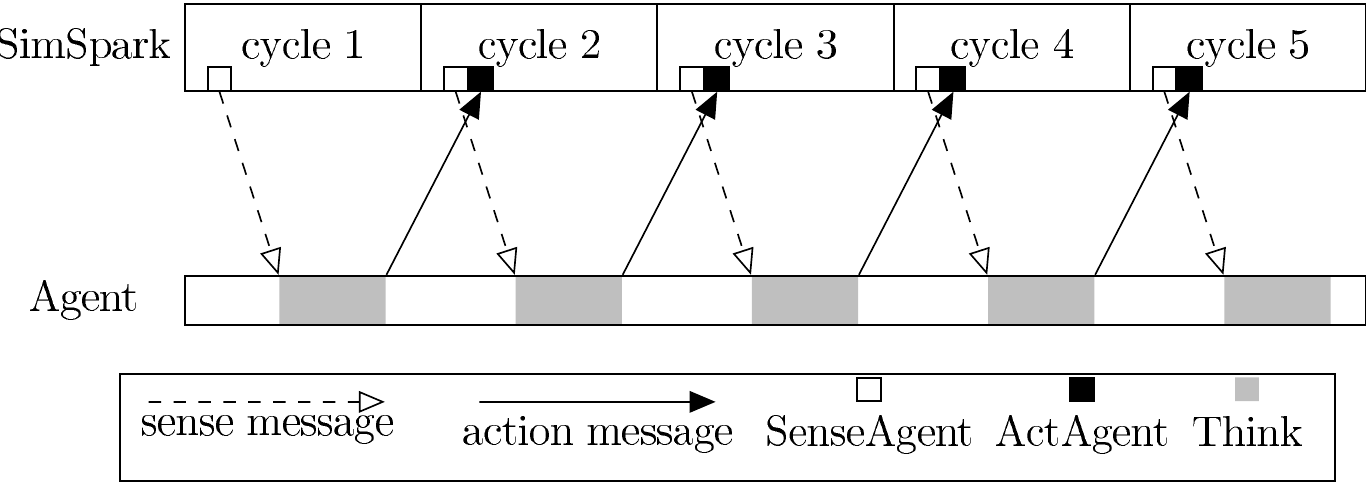
\includegraphics[width=0.8\textwidth]{Chapter3/figures/SimulationUpdateLoopSynchronizationBetweenSimSparkAndAgent.png}
  \caption{Server and Agent Communication.}
  \label{fig:Simulation-Update-Loop}
\end{figure}



\section{Perceptions}
Perceptions in simulated soccer are quite different compared to those in  real soccer games. Agents do not have to process raw data coming directly from sensors, but rather listen to sensor and higher-level observation messages sent by the server at each cycle. These messages take the following form:

\begin{verbatim}
(time (now 46.20))(GS (t 0.00) (pm BeforeKickOff))(GYR (n torso)
(rt 0.00 0.00 0.00))(ACC (n torso) (a 0.00 -0.00 9.81))(HJ (n hj
1)(ax 0.00))(HJ (n hj2) (ax 0.01))(See (G2R (pol 14.83 -11.81 1.
08))(G1R (pol 14.54 -3.66 1.12)) (F1R (pol 15.36 19.12 -1.91))(F
2R (pol 17.07 -31.86 -1.83)) (B (pol 4.51 -26.40 -6.15)) (P (tea
m AST_3D)(id 8)(rlowerarm (pol 0.18 -35.78 -21.65)) (llowerarm (
pol 0.19 34.94-21.49)))(L (pol 8.01 -60.03 -3.87) (pol 6.42 51.1
90 -39.13 -5.17))(L (pol 5.91 -39.06 -5.11) (pol 6.28-29.26 -4.8
8)) (L (pol 6.28 29.34 -4.95)(pol 6.16 -19.05 -5.00)))(HJ(n raj1
) (ax -0.01))(HJ (n raj2) (ax -0.00))(HJ (n raj3)(ax -0.00))(HJ(
n raj4) (ax 0.00))(HJ (n laj1) (ax 0.01))(HJ (n laj2) (ax 0.00)) ...\end{verbatim}

\noindent
The above message is an example message our agent has received from the simulation server during simulation. It includes information about the server time, the game state and time, values for each one of the joints, visual observations from the camera, and data from acceleration, gyroscope, and force sensors. We parse these messages and save the enclosed information in data structures appropriate for each type of perception. 

%Figure~\ref{fig:BeliefsUpdate} illustrates this procedure.
%\begin{figure}[t!]
%\centering
%  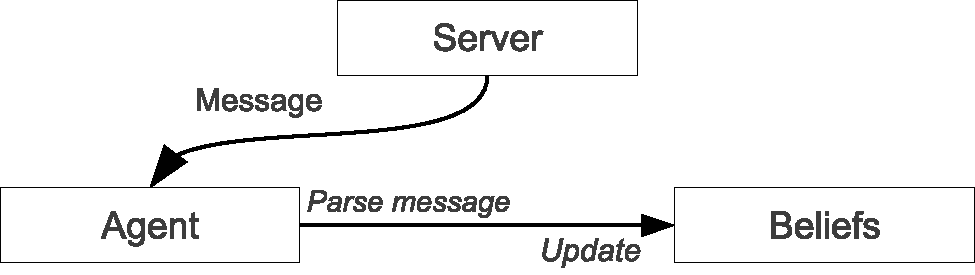
\includegraphics[width=0.8\textwidth]{Chapter3/figures/Message.pdf}
%  \caption{Beliefs Update.} 
%  \label{fig:BeliefsUpdate}
%\end{figure}


\section{Localization}
Once we have all the new perceptions from the server available, we can update our agents' belief about its current location in the field. A brief description of the localization process follows.

\subsubsection*{Self-Localization Process} 

Our localization scheme is largely based on a method proposed by a colleague within a common course project~\cite{Localization}. Localization, as a process, is executed every three cycles (60ms), in fact every time we receive observations from the vision perceptor. The potentially visible objects in our current field of view may be of different types: ball, landmarks, teammates, and opponents. After registering all currently visible objects, we use only the landmarks, which are found in permanent known positions in the field, to find candidate positions and update the agent's belief about the current position and orientation in the field. 

A key restrictive factor is that the agents are equipped with a restricted vision perceptor which limits the field of their view to 120 degrees. An example of this limitation is shown in Figure~\ref{fig:fieldofview}. It is easy to realize that the localization process would have been easier, if there was an omni-directional vision perceptor.

\begin{figure}[t!]
\centering
  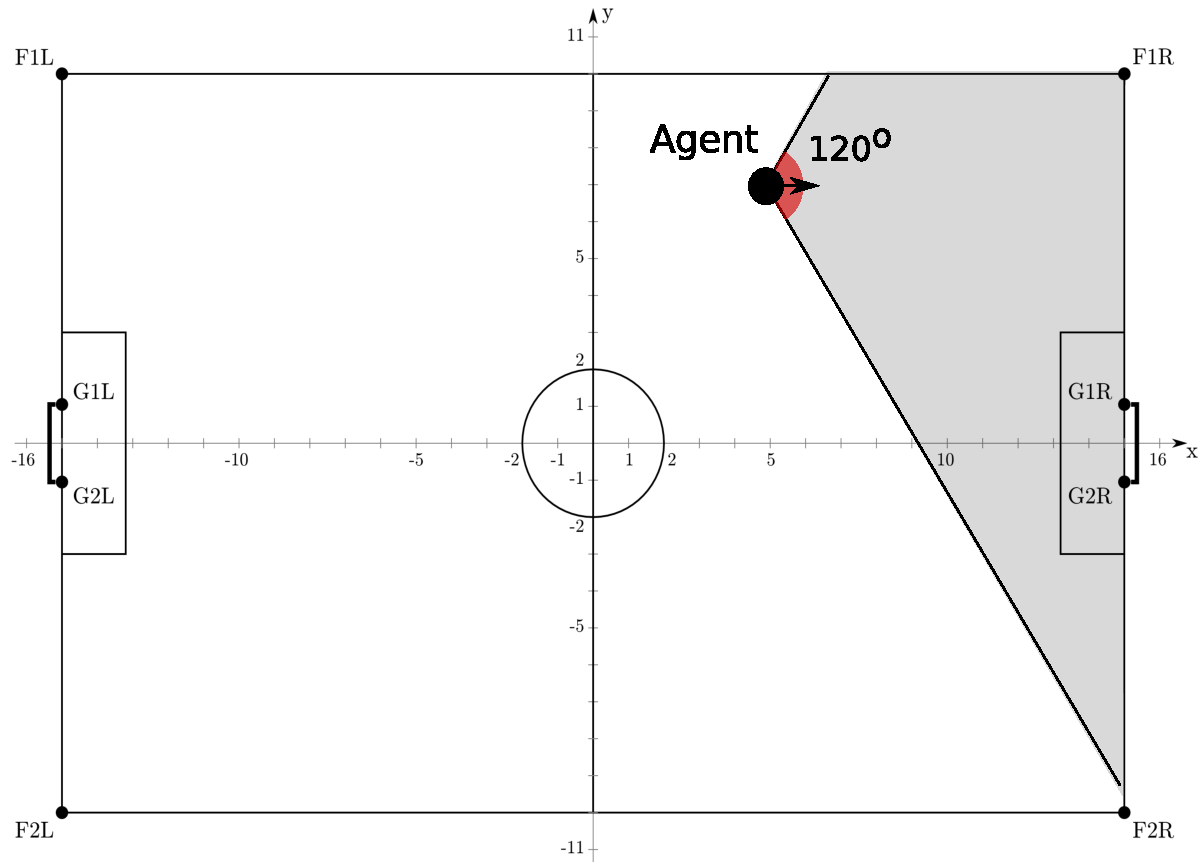
\includegraphics[width=0.8\textwidth]{Chapter3/figures/LViewAngle.pdf}
  \caption{Nao's Restricted Field of View.} 
  \label{fig:fieldofview}
\end{figure}
 
Localization process became possible through two main functions. The first function, takes the distance, as well as, horizontal, and vertical angles of two visible landmarks as arguments and returns as an output, a possible coordinate-$(x,y)$ and the orientation of the body in relation to the angle system of the simulation soccer field. These two landmarks form two circles with radius equal to the distance we see each of them and center the static and known coordinate of these landmarks. Obviously, these two circles intersect at 2 points. We keep as a final result the point which is within field's limits, rejecting the other. In cases where the agent sees more than two landmarks, this position is computed for every combination of two from all landmarks. Finally, an average position is calculated taking into consideration all output positions of this function. As we can realize, in cases where the agents has less than two visible landmarks in the field of their view, they are not able to compute a new observation. Figure~\ref{fig:Localization} presents the visual representation of this procedure. 

\begin{figure}[t!]
\centering
  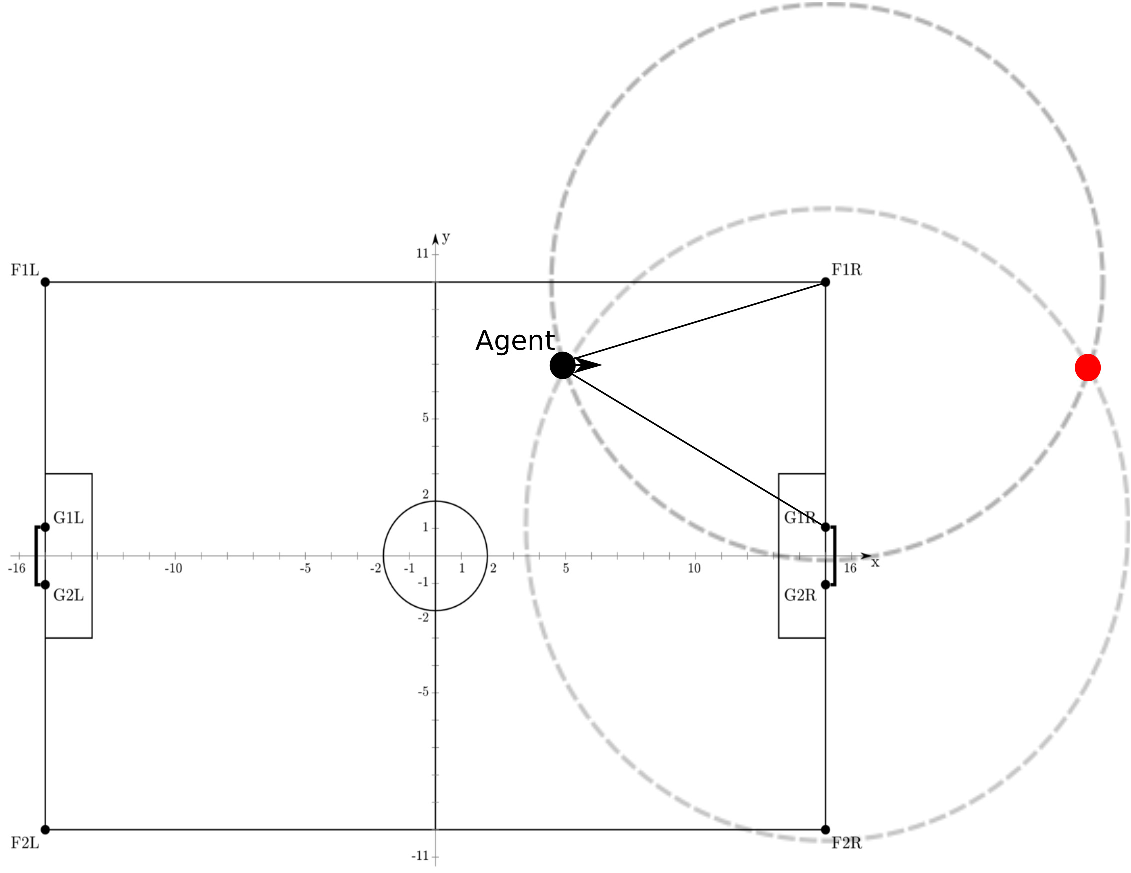
\includegraphics[width=0.8\textwidth]{Chapter3/figures/Localization.pdf}
  \caption{Localization Main Function.} 
  \label{fig:Localization}
\end{figure}

Except from the calculation of agent's position into the soccer field, the second function of the localization process is responsible to compute the position of the other visible objects such as other players and the ball. 
Knowing our position helps us locate other visible objects too. For every object which is located in our field of view, vision perceptor informs us about its vertical angle, its horizontal angle and its distance from our vision perceptor. This information is enough for the calculation of their exact positions into the field's coordinate system. Finally, after the localization process ends, we are able to have the following observations:

\begin{description}
	\item[Our Position] Only if agents see more than one landmarks.
	\item[Other Agents Positions] Only if agents know their positions and other agents are located in the field of their view.
	\item[Ball Position] Only if agents know their positions and ball is visible to them.
\end{description}
Figure~\ref{fig:LocalizationResults} presents the results which are computed by the localization process.

\begin{figure}[t!]
\centering
  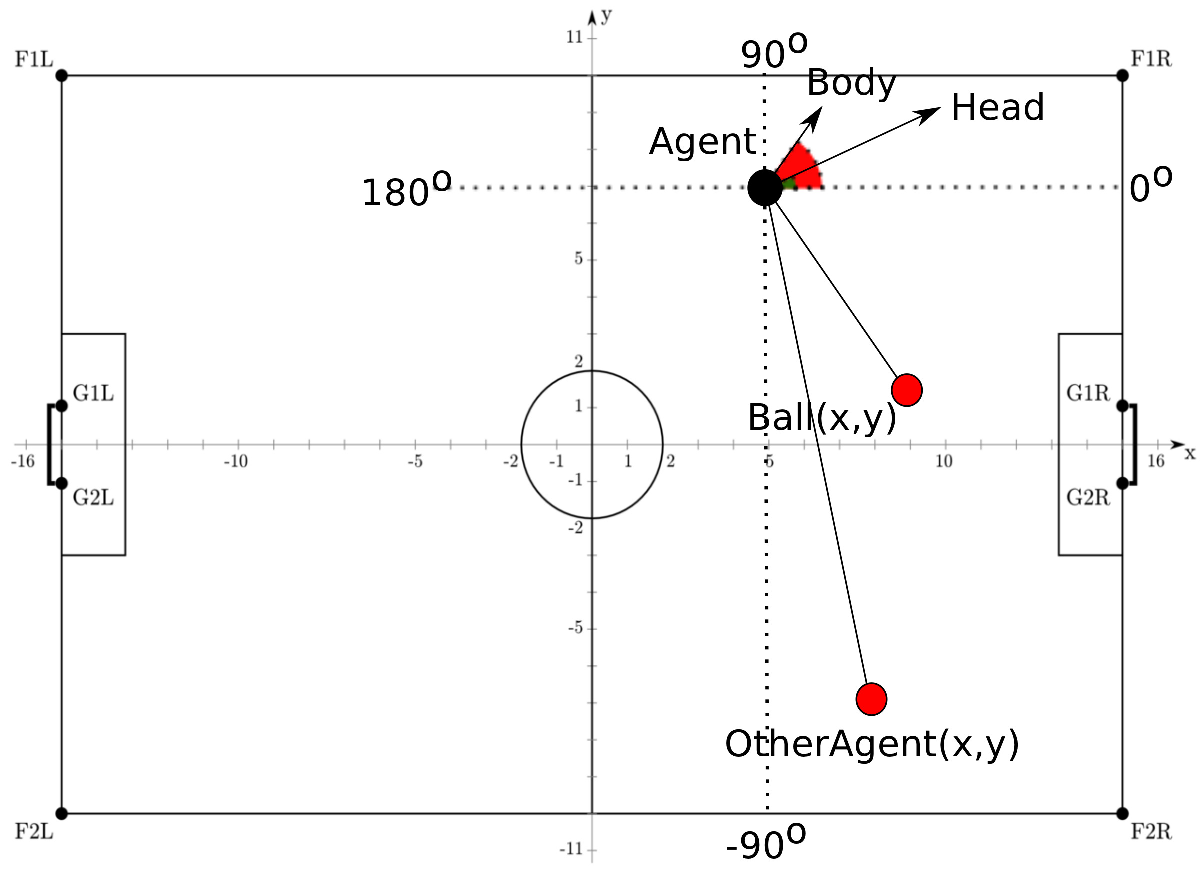
\includegraphics[width=0.8\textwidth]{Chapter3/figures/LocalizationResults.pdf}
  \caption{Localization Results.} 
  \label{fig:LocalizationResults}
\end{figure}
\hfill





\section{Localization Filtering}
In absence of a stochastic localization system, we are forced to ensure that localization results are qualitative enough for us to rely on. Due to symmetry of landmarks' positions and faulty observations due to noise existence, localization is not always accurate enough to depend on. Therefore, a kind of filtering is required for observations are computed by the localization process.

\begin{algorithm}[ht!]
\caption{Localization Filtering}
\label{LocalizationFiltering}
\begin{algorithmic}[1]
\STATE {\bf Input: }$Observation$
\STATE {\bf Output: }$FilteredPosition$
\IF{$size(Queue) = 0$}
\STATE $Queue.Add(Observation)$
\STATE $MyPosition = AVG(Queue)$
\ELSIF{$size(Queue) < MaxSize$}
\IF{$Observation \not\approx AVG(Queue)$}
\STATE $Queue.Remove()$
\ELSE
\STATE $Queue.Add(Observation)$
\STATE $MyPosition = AVG(Queue)$
\ENDIF
\ELSE
\IF{$Observation \not\approx AVG(Queue)$}
\STATE $Queue.Remove()$
\ELSE
\STATE $Queue.Remove()$
\STATE $Queue.Add(Observation)$
\STATE $MyPosition = AVG(Queue)$
\ENDIF
\ENDIF
\end{algorithmic}
\end{algorithm}

Algorithm \ref{LocalizationFiltering} describes the process of localization filtering. In general, localization process provides agents hundreds of observations about their location. The general idea we follow, is the fact that these observation do not include consecutive faulty observations. Therefore, it will be easy for us not to take into consideration updating agents' belief the observations that may seem faulty. 

To overcome this difficulty, we came up with a simple algorithm. The average of a queue full of observations always gives us our agent's position into the field. When an observation comes from the localization process, we check if the queue is empty or full; If it is empty, we just add the observation into the queue. If it is full of elements, then we check if the new observation seems faulty in comparison to the computed average of this queue. If it does, we do not take it into account and we just remove the last-inserted element. If not, then we add this position to the queue.
If queue is neither empty nor full, we make the same procedure checking if current observation is a faulty or not, with the only difference that we do not remove any element if it is not. Localization filtering applies for both the calculation of our agent's position and the ball's position. Its result was the improvement of the localization results in an adequate degree in order to rely on with confidence. This filtering, smooths the results of our belief's position and rejects most faulty observations.





\section{Motions and Movement}
\label{Motions}
In robotics, we define a motion as a sequence of joint poses. A pose is a set of values for every joint in the robot's body at a given time. Simulated Nao has 22 degrees of freedom, meaning to 22 hinge joints. Figure~\ref{fig:NaoAnatomy} shows Nao's anatomy.
For example, for a given set of n-joints a pose is defined as:\\
\begin{center}
$Pose(t)$=$\lbrace J_{1}(t),J_{2}(t),...,J_{n}(t) \rbrace$\\
\end{center}


\begin{figure}[t!]
\centering
  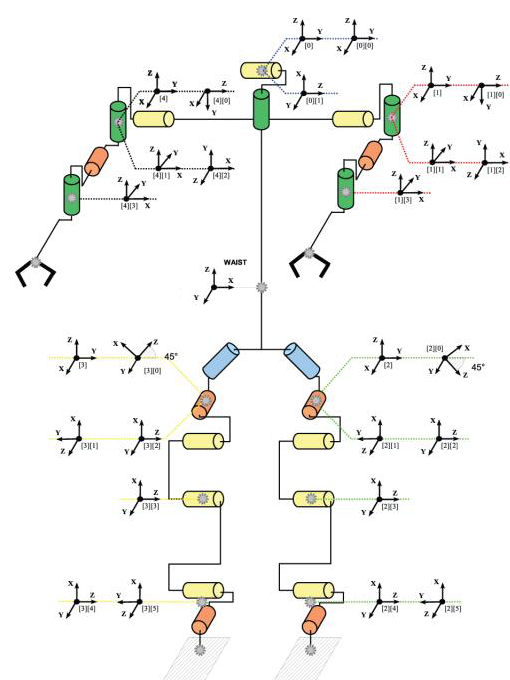
\includegraphics[width=0.3\textwidth]{Chapter3/figures/Models_NaoAnatomy.png}
  \caption{Nao's anatomy.}
  \label{fig:NaoAnatomy}
\end{figure}



Motions are very important part for every team taking part into the RoboCup simulation league. Most of the teams in this league, make use of dynamic movement which is a major advantage for their side. In this approach, we are using motion files. Motion files are set of poses which has standard values for each joint in every type of movement. The difference between static motion files and dynamic movements is that dynamic movement make use of direct and inverse kinematics as well as the computation of the center of the robot's body mass. This dynamically computed movements give robot better body balance and fast movement. In this approach, we are using two kinds of static motion files. Text based and XML based motion files.


\subsection{XML-File Based Motions}
These motion files has been created and used by FIIT RoboCup 3D project. They have XML structure and it was easy for us to implement them into our project. Structure of these xml motion files is shown below.
\begin{verbatim}
		<phase name="Start" next="Phase1">
			<effectors>
				Joint Values
			</effectors>
			<duration>duration</duration>
		</phase>
		
		<phase name="Phase1" next="Phase2">
			<effectors>
				Joint Values
			</effectors>
			<duration>duration</duration>
		</phase>
		
		<phase name="Phase2"next="Phase1">
			<effectors>
				Joint Values
			</effectors>
			<duration>duration</duration>
			<finalize>Final</finalize>
		</phase>
		
		<phase name="Final">
			<effectors>
				Joint Values
			</effectors>
			<duration>duration</duration>
		</phase>
\end{verbatim}
As we can realize by the structure of this xml file, each movement is split into phases. Each phase has a duration and joint values for every joint of the robot related to the movement. Moreover, every phase has an index which points to the next phase. For example, the first phase: ``Start'' has an index for the next phase: ``Phase1''. Phases with a finalize field help us to end each movement. For example, the phase: ``Phase2'' has a finalize index which points to the phase: ``Final'', this means that if we want to end the execution of this movement, we have to continue with the execution of the finalize phase and not with the next.
\subsection{XML-File Based Motion Controller}
Motion controller is a major component which controls and enables the movement ability of the robot. It is responsible for handling the movement requests by the agent. Agent has not access in motion controller itself but only has access in the motion trigger. We could describe this trigger as a variable which can only be changed by the agent. Each agent declares in this field the movement he is willing to perform. In each cycle, the motion controller reads this variable and generates a hinge joint effector string which is the result of its process.


\begin{figure}[t!]
\centering
  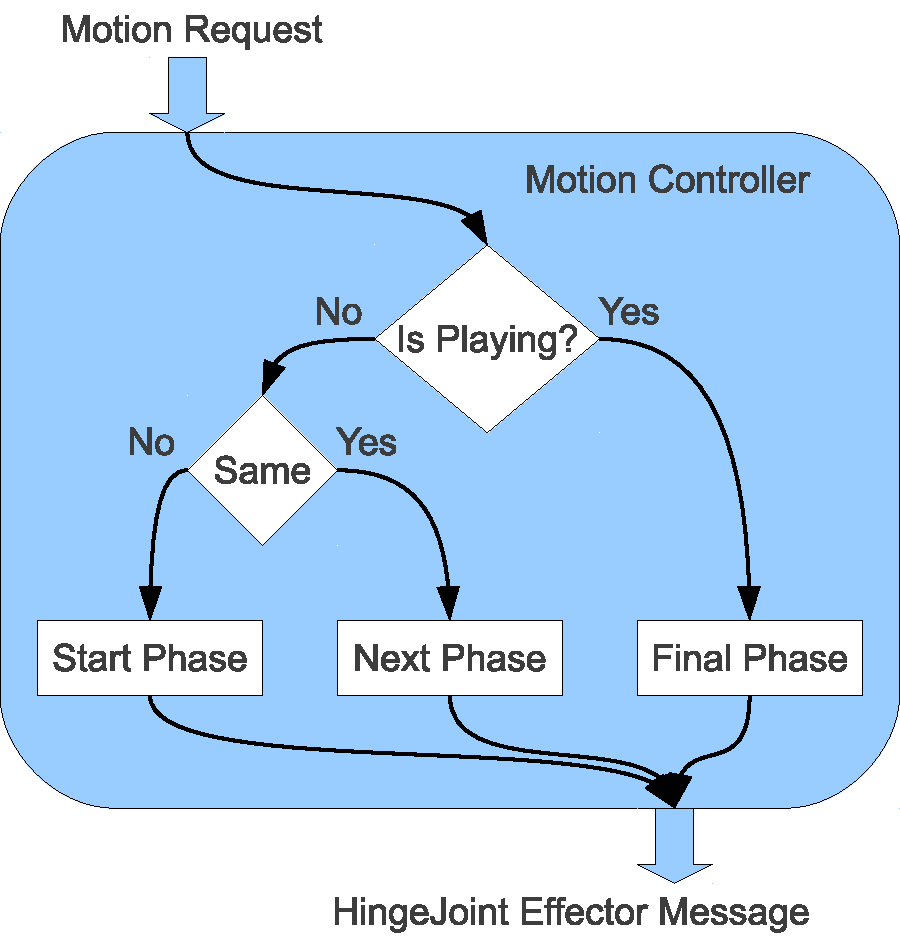
\includegraphics[width=0.6\textwidth]{Chapter3/figures/MotionController.pdf}
  \caption{Motion Controller.}
  \label{fig:MotionController}
\end{figure}


Figure~\ref{fig:MotionController} describes the general architecture of the motion controller. Motion controller checks if there is a motion which is playing already. If   already playing motion is the same as the requested one, motion controller continues with the next of its phases, if not, controller tries to finalize the playing movement in order to start playing the new requested one.


\begin{figure}[t!]
\centering
  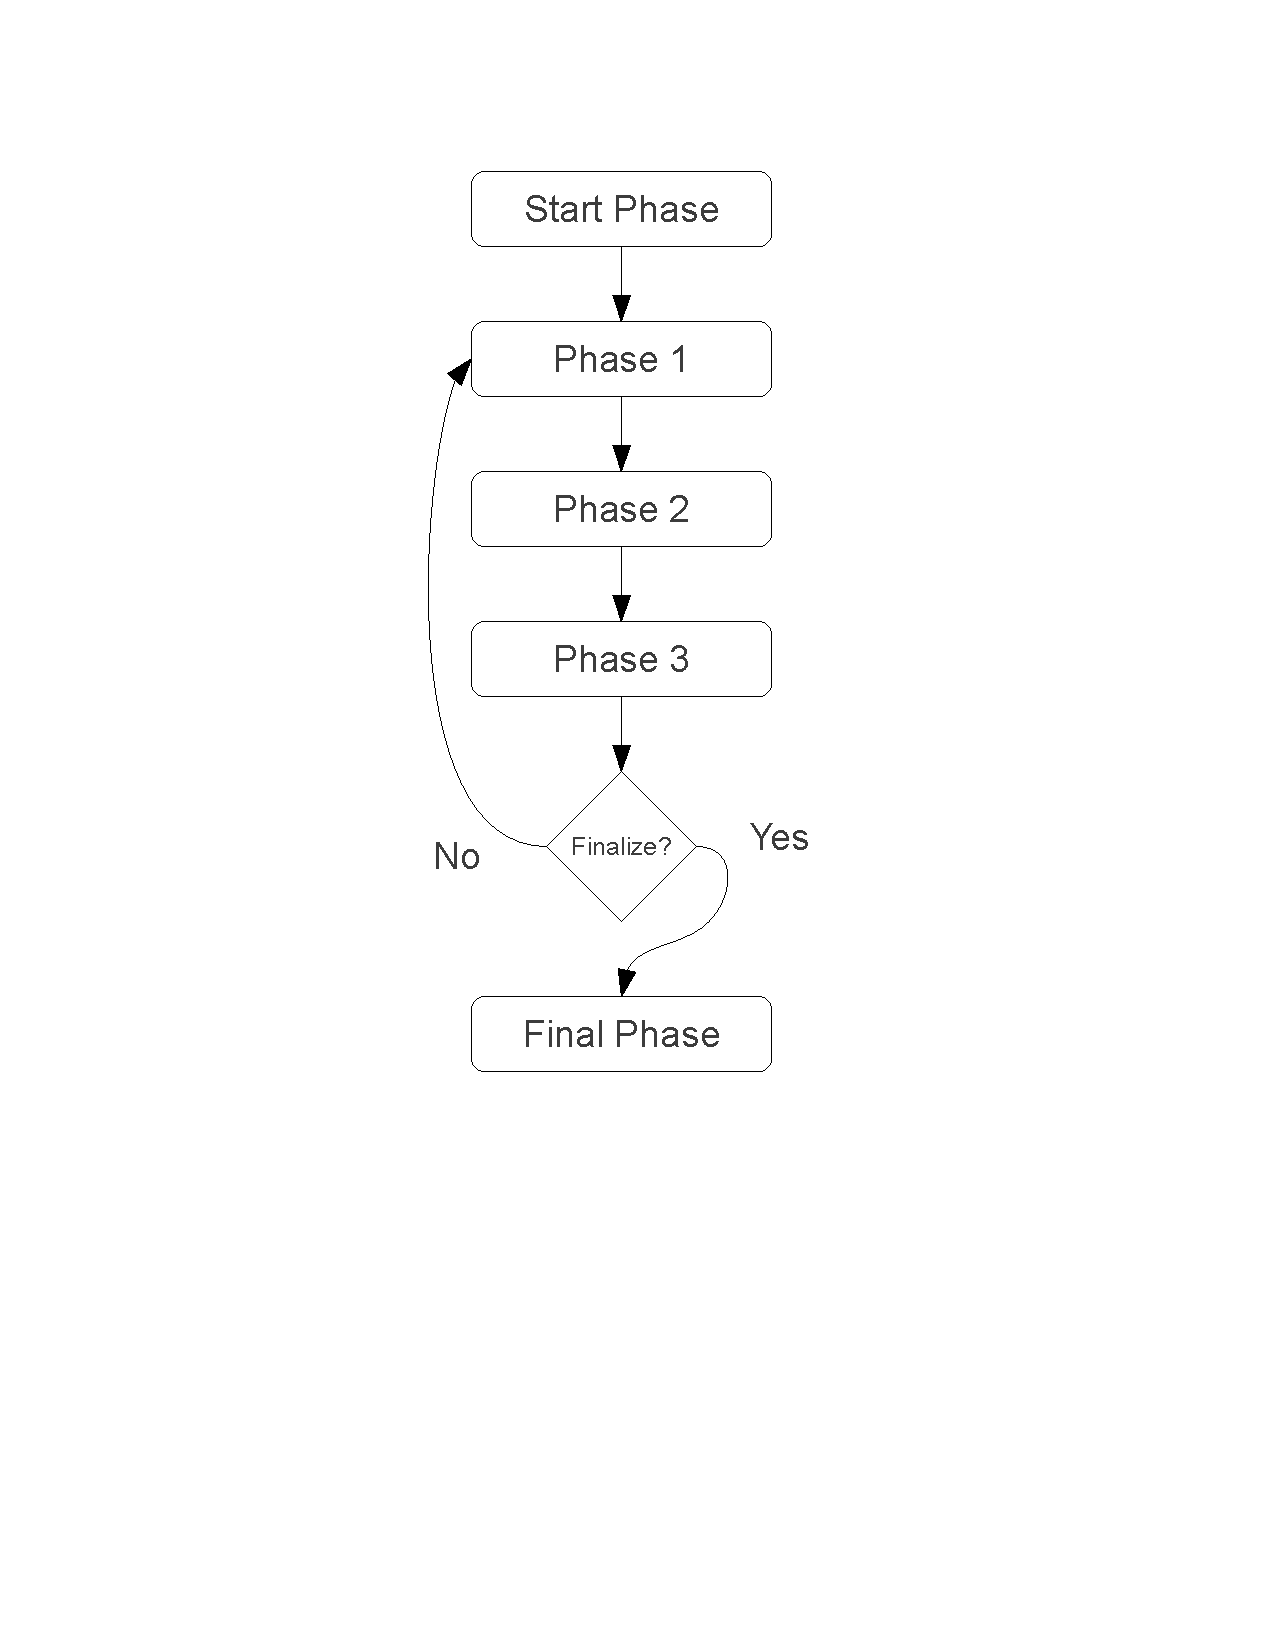
\includegraphics[width=0.2\textwidth]{Chapter3/figures/MotionSequence.pdf}
  \caption{Phase Sequence.}
  \label{fig:PhaseSequence}
\end{figure}


Figure~\ref{fig:PhaseSequence} describes the exact motion sequence. In general, XML motions is created to include cycles. For example, walking motion has three main phases which create a cycle. If motion trigger has not changed at the last phase, we have to continue with the execution of the first phase not with the final one. As we saw in the structure of every XML based motion file, each phase has a set of joint values. These values are in degrees. To generate motions for our agent we need to create a motion string. This string encloses information about each joint's velocity. This velocity can be computed by:
\begin{center}
$Axis Change = Already Joint Value - Desired Joint Value$
\end{center}
Having each joint's desired axis change and the duration of this phase in seconds. We can compute, how much will be the speed of every joint in order to reach to the desired joint value in this time limit.
\begin{center}
$Velocity = \frac {Axis Change} {PhaseDuration} $ Degrees/Sec
\end{center}
This velocity is computed for every involved joint in the motion. The final output of the motion controller will be send to the server. In addition, we include in this message zero velocity for every joint which is not included in the \texttt{effector} field of each phase.



\subsection{Text-File Based Motions}
The other kind of motion files we are using is used by Webots simulator. These text based motion files have simpler structure than the XML motion files. In default, each pose lasts for two simulation cycles (40ms). Structure of these motion files is shown below.
\begin{verbatim}
#WEBOTS_MOTION,V1.0
LHipYawPitch,LHipRoll,LHipPitch,LKneePitch,LAnklePitch,...
00:00:000,Pose1,0,-0.012,-0.525,1.05,-0.525,0.012,0,...
00:00:040,Pose2,0,-0.011,-0.525,1.05,-0.525,0.011,0,...
00:00:080,Pose3,0,-0.009,-0.525,1.05,-0.525,0.009,0,...
00:00:120,Pose4,0,-0.007,-0.525,1.05,-0.525,0.007,0,...
00:00:160,Pose5,0,-0.004,-0.525,1.05,-0.525,0.004,0,...
00:00:200,Pose6,0,0.001,-0.525,1.051,-0.525,-0.001,0,...
00:00:240,Pose7,0,0.006,-0.525,1.05,-0.525,-0.006,0,...
00:00:280,Pose8,0,0.012,-0.525,1.05,-0.525,-0.012,0,...
00:00:320,Pose9,0,0.024,-0.525,1.05,-0.525,-0.024,0,...
\end{verbatim}
At the second row, all joints which involved in the specific movement are defined. As an example, walking motion requires joints from both robot's legs only. The above rows from left to right have information for the duration of each pose, the pose number and finally desired angles for each joint in radians in the same order as they were defined in the second row.


\subsection{Text-File Based Motion Controller}
Motion controller for text based motions is based on the same principle as the XML controller. The joint values in the motion files represent radians. So, we have to convert these values into degrees and then we proceed with the next steps. Each pose lasts for one or two cycles depending on the speed we want each motion to be executed. This motion controller could be customized easily to perform motions in different ways. There are parameters which can be changed such as:
\begin{description}
	\item[Duration] How many cycles from pose to pose.
	\item[Pose Offset] Pose Offset = 2, we execute pose1,pose3,pose5,...
	\item[Hardness Factor]Hardness Factor = 0.9, we multiply velocity with this factor.
\end{description}
The desired velocity of every joint is computed by:\\
\\
$Axis Change$ = $Already Joint Value$ - $RadiansToDegrees(Desired Joint Value)$
\\
\\
$Velocity = (\frac {Desired Axis Change} {Duration
 \ast CycleDuration})\ast Hardness Factor$ $Degrees/Second$\\
\\
This velocity is calculated for every involved joint in the motion. The final output of the motion controller will be send to the server.

\subsection{Dynamic Elements in Movement}
In contrast with the general idea about static motion files stated in the beginning of this Section~\ref{Motions}, we have tried to implement some dynamic features in our movements. There is not so much room for improvement in these static motions but we managed to achieve nice results.
\begin{description}
	\item[Walk Leaning] Walking can lean to the right and to the left. There was an improvement on overall performance as agent should not be forced to turn his body in every occasion, even if the target angle is small.
	\item[Walk Slowdown] Its important our agent to slowdown his speed in order to stop his body with more stability.
	\item[Turn]	Agent turns its body as much as it need from 7 to 40 degrees. Figure~\ref{fig:Turn} shows this process. X-axis presents the hardness factor, and Y-axis presents how much each motion turns the body of the agent for each hardness factor value in degrees.
\end{description} 


\begin{figure}[t!]
\centering
  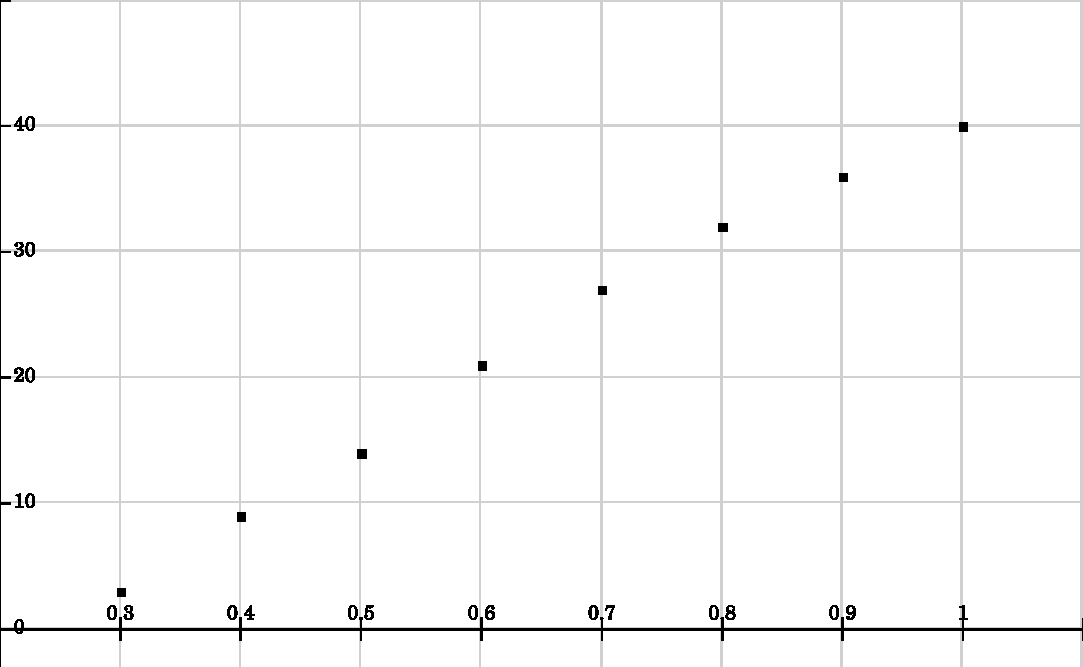
\includegraphics[width=0.8\textwidth]{Chapter3/figures/DynamicTurn.pdf}
  \caption{Dynamic Turn, Degrees (y-axis), Hardness Factor (y-axis).}
  \label{fig:Turn}
\end{figure}


\section{Actions}
In this section, we describe the way that agents can affect and change their environment. In general, action is the result of the agent's perception in combination with its procedure of thinking. In our approach, actions are split into groups in terms of their complexity and type.

\subsection{Simple}
Simple actions make use only of movements and have a simple structure. These simple actions are:
\begin{description}
 \item[Turn To See Ball] This action results in turning the agent until ball is in the field of its view.
 
 \item[Turn To Ball] This action turns agent towards the direction of the visible ball. It has prerequisite the above action.
 
 \item[Turn To Locate] This is the default action each agent does when he loses his position ( sees less than two landmarks ). It helps agent to re-localize itself into the field.
 
 \item[Walk To Ball] Agent walks towards the ball. He stops when the ball is close enough to perform a kick for example. Remind, that distance from ball stems from vision perceptor and defines the distance between the agent's vision perceptor - which is attached to agent's head, and the ball. So, it is better for the agent to calculate the distance between its feet and the ball. This became feasible thought direct kinematics via trigonometry in 2-dimension space. Starting from agent's ankle as the starting point of both axis (0,0), it is easy to calculate every joint's position in 2D-space from ankle to head. Figure~\ref{fig:2dkinematics} shows how joint values are related with the feet's distance from the ball.
 
 \begin{figure}[t!]
\centering
  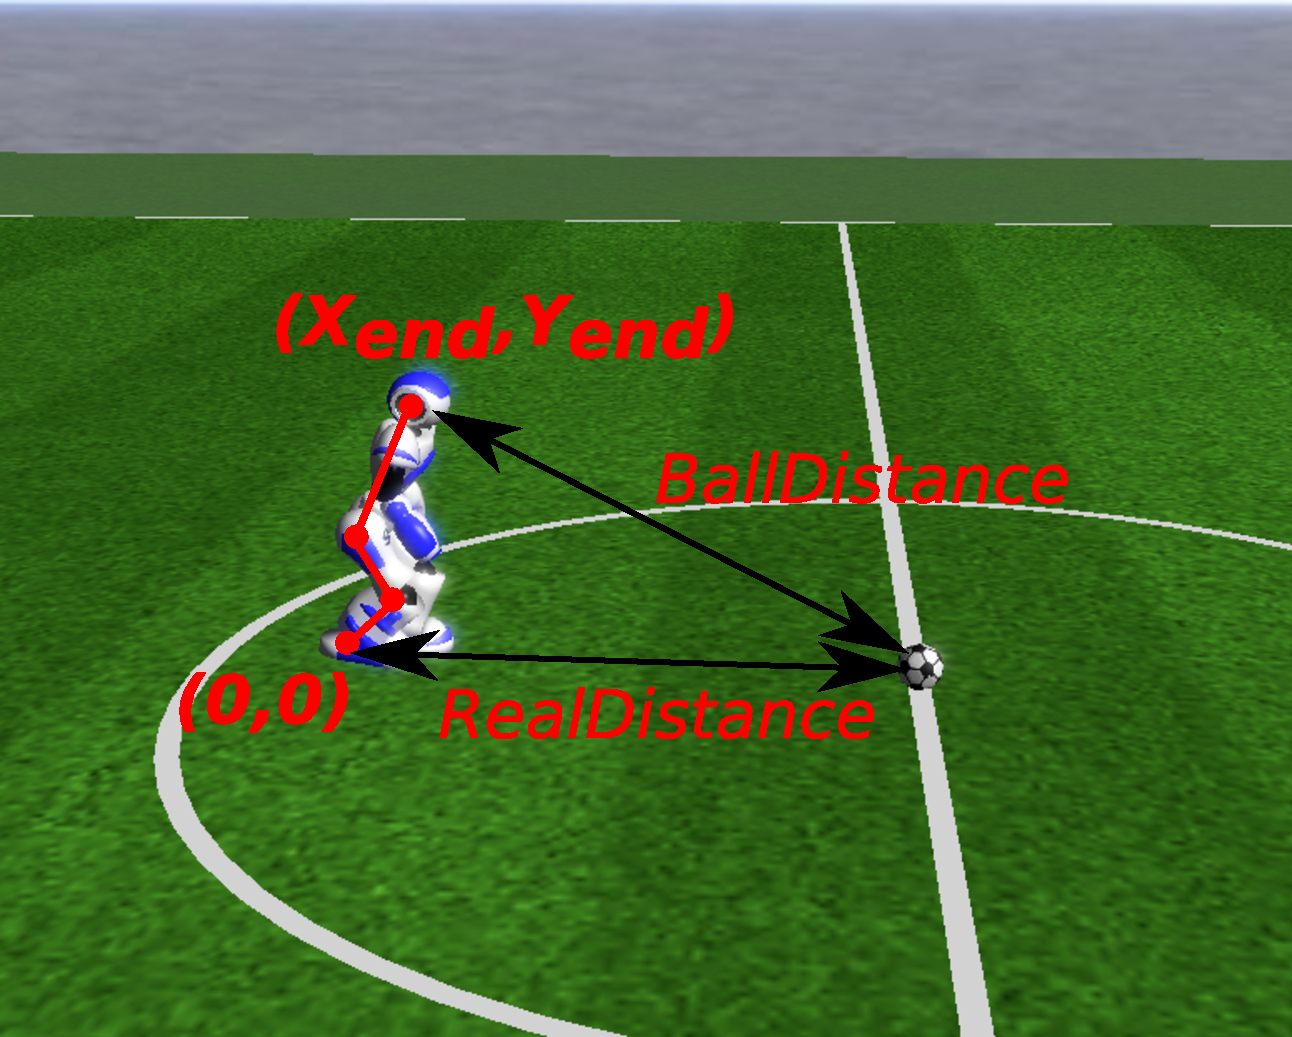
\includegraphics[trim=0cm 4cm 0cm 4cm, clip,width=0.8\textwidth]   {Chapter3/figures/2dkinematics.pdf}
  \caption{Ball Distance from Agent's Feet.}
  \label{fig:2dkinematics}
\end{figure}


 \item[Stand Up] Agent executes it when he is fallen on the ground in order to get up.
 \item[Prepare Kick] Agent executes it before performs a kick. This action is needed in order agent to have a proper position to kick ball successfully. Figure~\ref{fig:NaoKick} shows an example in which is shown the agent's position in relation to ball before a kick.
  
  
\begin{figure}[t!]
  \centering
  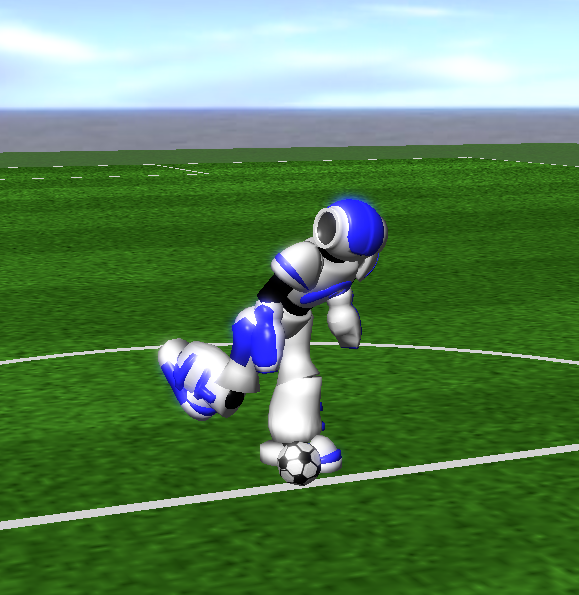
\includegraphics[trim=0cm 3cm 0cm 4cm, clip,width=0.6\textwidth]{Chapter3/figures/NaoKick.png}
  \caption{Nao Before Kick Ball.}
  \label{fig:NaoKick}
\end{figure}
\end{description}



\subsection{Complex}
Complex actions are created to make use of more than one simple actions and motions, they have a more complicated structure. These complex actions are:
\begin{description}
 \item[On Ball Action] This action uses and has the necessity for the successful execution of Walk To Ball action in order the agent to reach the ball. In this action we use the agent's belief about his location in the field as well as, data coming from vision perceptor directly to help us find the direction towards the opponents' goal and the kick's type. This action has a finite state machine logic. Figure~\ref{fig:GoKickBallToGoal} shows in what order this action is executed. In every state it is possible an opponent agent takes the ball away from the agent. In this situation agent returns to its initial state.


 \begin{figure}[t!]
\centering
  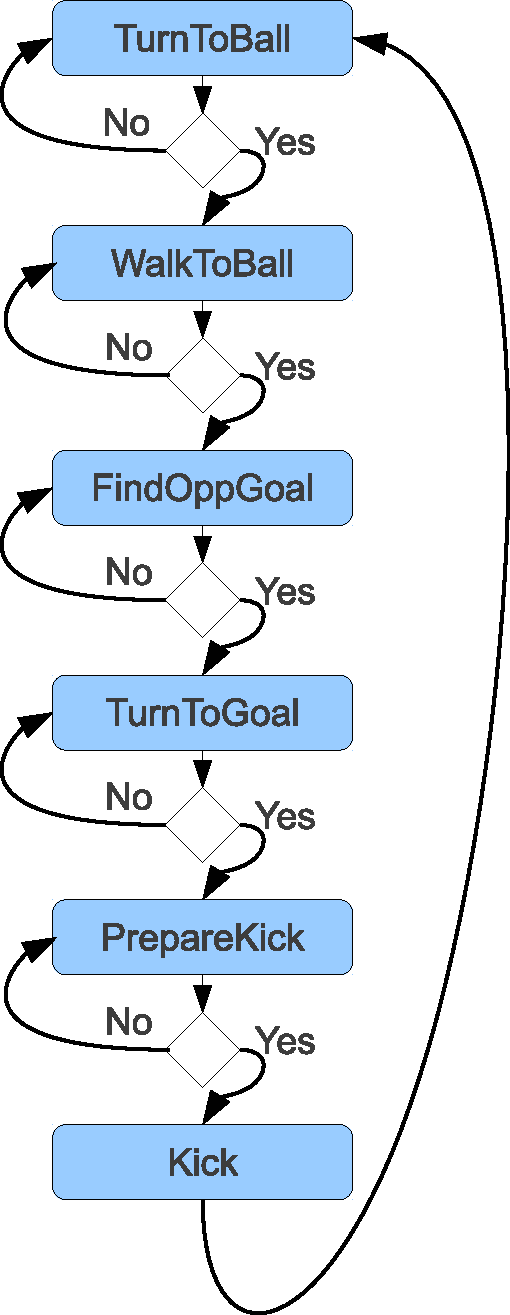
\includegraphics[width=0.25\textwidth]{Chapter3/figures/KickFSM.pdf}
  \caption{On Ball Action Logic Sequence.}
  \label{fig:GoKickBallToGoal}
\end{figure}



 \item[Walk To Coordinate]
 This action leads agent to a specific coordinate-$(x, y, theta)$ in the soccer field. To achieve this action we need to know our position and the target coordinate and target orientation. Knowing our position, it is easy for agent to calculate in which direction has to walk in order to reach the specific coordinate. Figure~\ref{fig:WalkToCoordinate} shows in what direction agent should walk from the point $(X_{start},Y_{start})$, to the point $(X_{target},Y_{target})$. $\vartheta_{target}^{\circ}$:\\
\begin{center}
$d_{X} = X_{target} - X_{start}$\\
$d_{Y} = Y_{target} - Y_{start}$\\
$\vartheta_{target}^{\circ} = atan2(d_{X},d_{Y})$\\
$d_{target} = \sqrt{d_{X}^2 + d_{Y}^2}$
\end{center}
Been helped from the above calculations agent is always aware of the distance and the direction it has to travel towards its target position. 


 \begin{figure}[t!]
\centering
  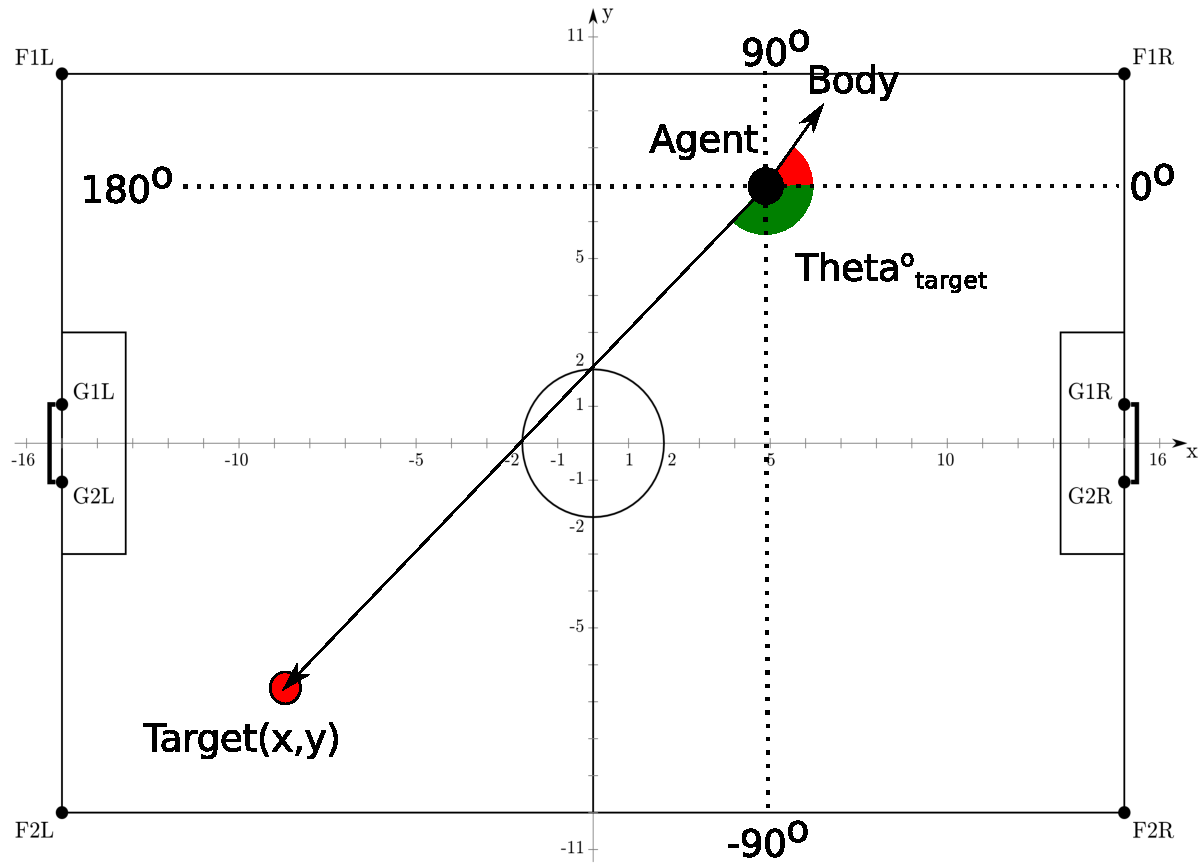
\includegraphics[width=0.8\textwidth]{Chapter3/figures/GoToPos.pdf}
  \caption{Walk To Coordinate Action.}
  \label{fig:WalkToCoordinate}
\end{figure}


 \item[Walk To Direction]
 This action leads agent to walk towards a specific direction.
 
 \item[Walk With Ball To Direction]
 As far as agent reaches the ball, he will try to keep the ball in front of its feet and walk towards a direction keeping into mind that the ball has to be always in front. This action is not yet functional in our approach as movements based on motion files make it hard for us keeping ball in front of our agent all the time.
 
\end{description}

\subsection{Vision}
Vision-related actions were created to control the vision perceptor which is attached to the robot's head as well as to collect data from it in order to execute related actions such as obstacle avoidance. These vision related actions are:
\begin{description}
 \item[Head Movement] This action is related with the movement of the head in different occasions. Nao robot has two joints attached in the neck which give us enough freedom to move its head in relation to the action is being performed.
 \begin{description}
 
 \item[type 1] Head is moving to its original position. Both joint-axis are given $0$ degrees as desired angles.
 
 \item[type 2] Head is moving until agent see the ball.
 
 \item[type 3] Head is moving in relation to the ball's movement. In this type head follows the ball movement in condition that head does not exceed both axis thresholds.
 
 \item[type 4] Head is doing a harmonic movement in order agent to have a nice perception of its environment. This type of head's movement is used in obstacle avoidance and walk to coordinate actions.
 
 \item[type 5] Head is moving until agent can localize himself in the field.
 
 \end{description}
 
 \item[Watch Object Movement] This action requires that object is in agent's field of view. Computing the direction and the speed of the moving object is only feasible if we keep in memory a short number of observations. We keep two sets of five observations which we have taken within a time offset. Finding the average position of each set gives a distance between these two positions. If this distance will be divided with the time difference of the two observation sets we are going to have the direction and the speed of the moving object.
 
 
 \item[Find Opponents Goal] This action is used in On Ball action in order to take observations about the direction of the opponents goal in relation to agent's body angle.
 
 
 \item[Percept Obstacles]
 An action that has the responsibility of having a good view of all obstacles which are located in agent's close range. Due to the fact that simulated Nao's head can move in horizontal axis from $120^{\circ}$ to $-120^{\circ}$ and our field of view is $120^{\circ}$ means that we can have a complete imaging from all obstacles which are located close to our agent.
So, in every cycle of Nao's head we store all obstacles in an array. It is usual to observe the same obstacle more than once, in this situation we compute the average of these observations. At the end of head's cycle we call the main obstacle avoidance action which is going to find alternative routes if there is an obstacle in our way.


 \item[Obstacle Avoidance]
 In a dynamic and a multi-agent environment like simulation soccer this action is more than necessary. However, there are some teams in simulated soccer competition which have not develop an obstacle avoidance system yet. In our framework there is a
 reliable and a well-tested system to avoid possible collisions with other agents as well as landmarks (goal-posts).
 
 
  \begin{figure}[t!]
  \centering
  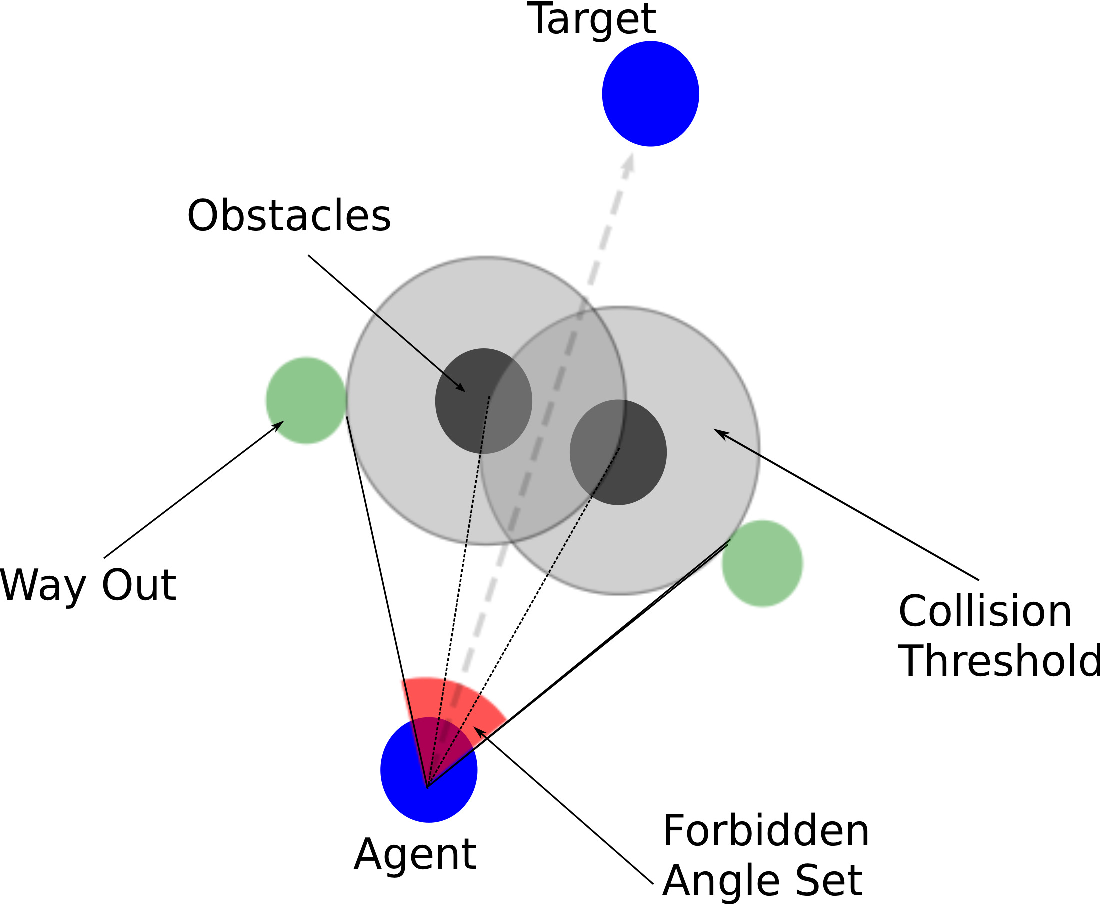
\includegraphics[width=0.6\textwidth]{Chapter3/figures/ObstacleAvoidance.pdf}
  \caption{Obstacle Avoidance.}
  \label{fig:ObstacleAvoidance}
\end{figure} 
\end{description}

Figure~\ref{fig:ObstacleAvoidance} presents an example in which there are two obstacles between the agent and its target position. During its walking agent scans the field for possible obstacles through the action mentioned above. If agent realizes that there is an object which blocks its way to the target in the same simulation cycle he starts computing the possible way out angles that it can choose in relation to its observations about all obstacles. For every obstacle, we calculate a set of two angles. These angles are determined by the distance between the agent and the obstacle and they imply in which direction we can avoid this obstacle. When these angles are calculated, we check every angle of each set if it belongs to another angle set too. Angles which belong to another set are removed from the final list.

\begin{algorithm}[ht!]
\caption{Way Out Angle Set Computation}
\label{AngleSet}
\begin{algorithmic}[1]
\STATE {\bf Input: }$Obstacles = \lbrace O_{1},O_{2},...,O_{n} \rbrace $
\STATE {\bf Output: }$WayOutSet[ ]$
\FOR{{\bf each} i in Obstacles}
\STATE $WayOutSet.Add(Calculate(O_{a},t)),\vee t \in \lbrace right,left \rbrace$
\ENDFOR
\FOR{{\bf each} j in WayOutSet}
\FOR{{\bf each} t in $\lbrace right, left \rbrace$}
\IF{$WayOutSet_{j,t} \in WayOutSet_{k}, \vee k \in \lbrace 1,2 \ast n \rbrace , k \neq j$}
\STATE $WayOutSet.Remove(j,t)$
\ENDIF
\ENDFOR
\ENDFOR
\end{algorithmic}
\end{algorithm}

This process' algorithm is described in Algorithm~\ref{AngleSet}. Once we have all the qualified angle sets from the algorithm, it is time to find coordinates which are safe in order to avoid one or more obstacles. For each angle in these sets we compute a specific coordinate. These coordinates in the soccer field will give us routes that are safe to follow. For every of these coordinates, we are going to calculate the cost of each route in respect to our body angle and the distance we have to travel to our target if we follow each of these routes. The route with the minimum cost is qualified and will be followed by the agent. Calculating this cost will give as dynamically consistent results meaning that if this function outputs a specific route at time $T$, assuming that obstacles are not moving, it will output the same route for every time $t > T$, until we will have a clear of obstacles route to our target position.


\subsection{Other Sensors}

Other Sensors related actions are created to collect data from gyroscope, accelerometer and force resistance perceptors. In this category there is only one action. This action is called {\bf Check If Fall} and is responsible for checking if our agent is fallen on the ground. In a multi-agent environment like soccer simulation league we should be aware about possible collisions with other agents or falls because the instability of certain movements. First of all, incoming perceptual inputs related to both gyroscope and accelerometer values are used to detect whether the robot has become subject of a turmoil or not. Taking values above a specific threshold from these two perceptors, it is possible that the robot has fallen, but we are not completely sure to perform a stand up action yet. It is not unusual to receive values above threshold due to a collision with an obstacle without a fall. So, we have to check the force resistance perceptors which are located on the sole of agent's feet. If these perceptors imply that the legs do not touch the ground then we are pretty sure to perform a stand up action.Foot pressure value is also used to determine whether the stand up action is succeeded.


\section{Communication}
Communication in Simspark is not ideal. There are not restrictions about the use of say effector and every agent can use it in every cycle. However, the hear perceptor comes up with some restrictions. Messages shouted from beyond a maximal distance (currently 50 meters) cannot be heard. Note that as the field is currently only 21x14(0.6.5) or 20x30(0.6.6) meters (25 or 36 diagonally), this does not turn out to be a limit in practice. Due to the limited communication bandwidth we utilize the communication channel in the following way, making sure that every message which is sent from an agent will be heard by other agents in time. A simple communication protocol is created in which time is sliced into pieces each one of them lasts one server cycle (20ms) and repeats every three cycles (60ms). Figure~\ref{fig:TimeSlicing} shows how time is sliced. Every three cycles there is one of these pieces in which only one agent is able to send its message to the others. Every slice has an integer label on it which states the uniform number of the player which is able to send its message. This label grows by one in every time a player send its message until it reaches the maximum uniform number, then it returns to the number one. Agents are not permitted to use a common chronometer for this task but we make sure that each player is synchronized with the others making use of the changing game states. By using this simple protocol we achieve that every player can receive the other eight agents' messages in 540ms.

\begin{figure}[t!]
\centering
  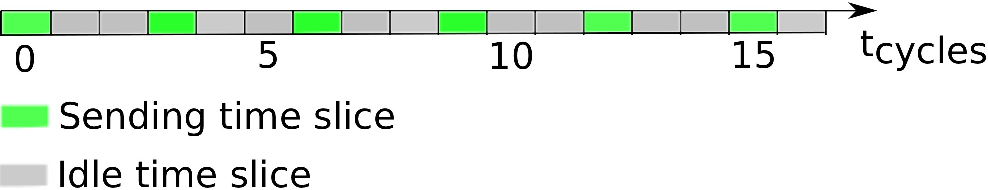
\includegraphics[width=0.8\textwidth]{Chapter3/figures/MAC.pdf}  
  \caption{Time Slicing Communication.}
  \label{fig:TimeSlicing}
\end{figure} 


\section{Goalkeeper Behavior}

In our approach, only goalkeeper ``runs'' an independent behavior, the rest field agents start a communication procedure between them and goalkeeper in order to inform him about their beliefs of the world state and their state whenever it is needed. Goalkeeper, is going to decide about the actions that every field player should do. So, we can realize that field players do not execute any behavior. In contrast, goalkeeper executes this task for them.

This section presents the behavior that leads goalkeeper to make decisions and choose actions for itself. As we said in Section \ref{Architecture}, goalkeeper is the only agent in our team who ``runs'' his own behavior. His behavior depends on a finite state machine. His initial state is ``\textbf{start}'' state. In this state goalkeeper tries to move himself in the center of his goal. When he accomplishes moving there, we change his FSM's state to ``\textbf{Guard}'' state. In guard state he makes use of the Watch Object Movement action to figure out the ball's current position and the  direction and the speed of its possible movement.

\begin{figure}[t!]
\centering
  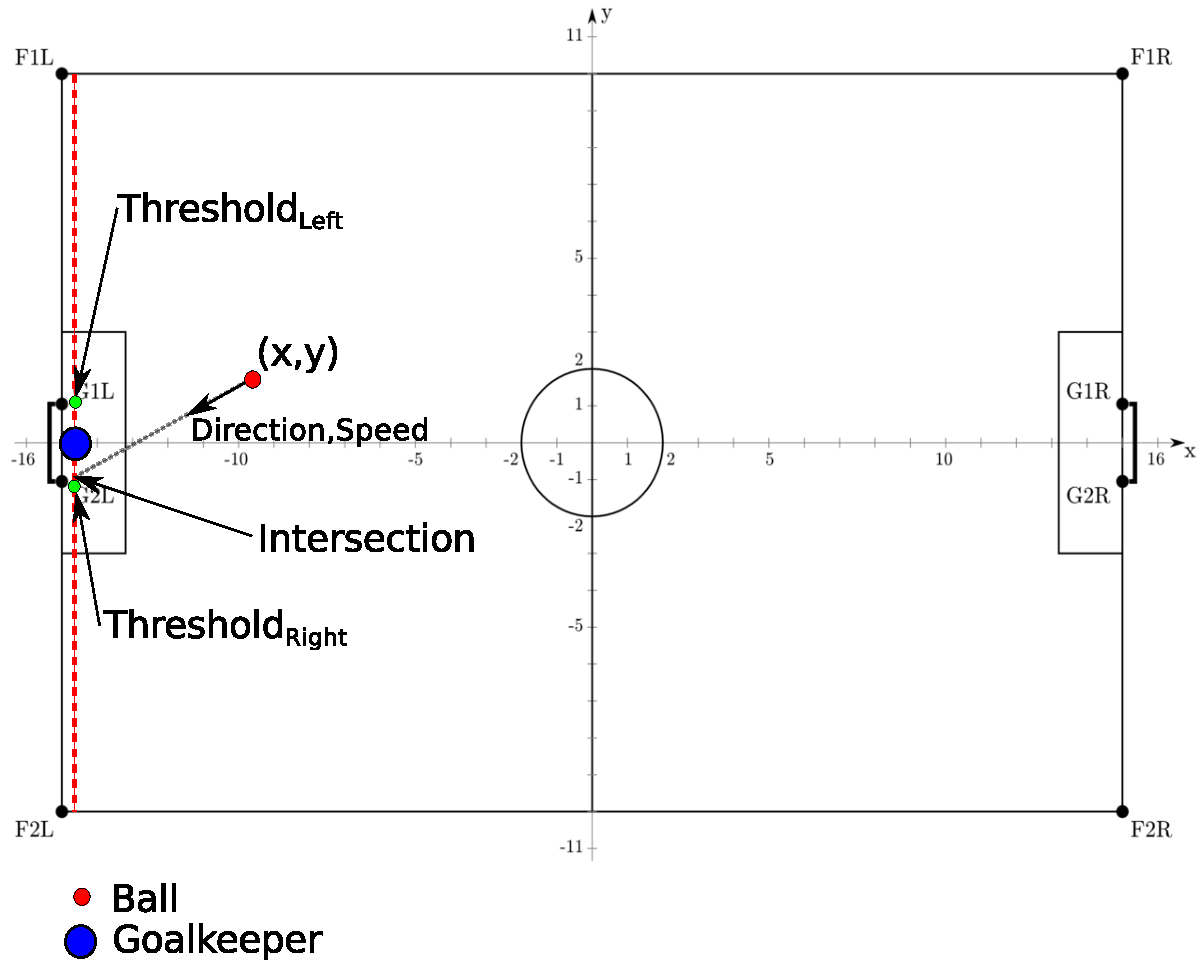
\includegraphics[trim = 0cm 0cm 10cm 0cm, clip,width=0.6\textwidth]{Chapter3/figures/Goalie.pdf}  
  \caption{Goalkeeper Fall Function.}
  \label{fig:Goalkeeper}
\end{figure} 

Figure~\ref{fig:Goalkeeper} is going to help you understand easier this state's basic idea. Goalkeeper Considers his position as the start of both axis x and y due to difficulties in making use of the localization process. So, red dashed line determines the goalkeeper's y-axis and x-axis. For every movement of the ball he tries to compute if there is an intersection point between its y-axis and the grey dashed line which starts from ball's position in the direction of ball's movement. If there is an intersection point between these two lines then agents computes if this point is out of the two thresholds ($Threshold_{Right}$,$Threshold_{Left}$). If not, we are pretty sure that ball is heading towards our goal. We compute how much time will take to the ball to meet our y-axis according to its speed and taking account the friction between ball and the ground. If this time is equal or less than the time takes our agent to fall, agent performs a right or a left fall. You can see agent falling to prevent a goal in Figure~\ref{fig:GoalkeeperFall}. There are also other states. State ``\textbf{Libero}'' is a state in which goalkeeper sees the ball into his box and there are no other agents near to it. Then goalkeeper goes to clear the ball from his box. Through coordination process informs other field players that he is at ``libero'' state to prevent them from going towards the ball too. When he clears the ball, he returns to his initial position. 

\begin{figure}[t!] 
\centering    
	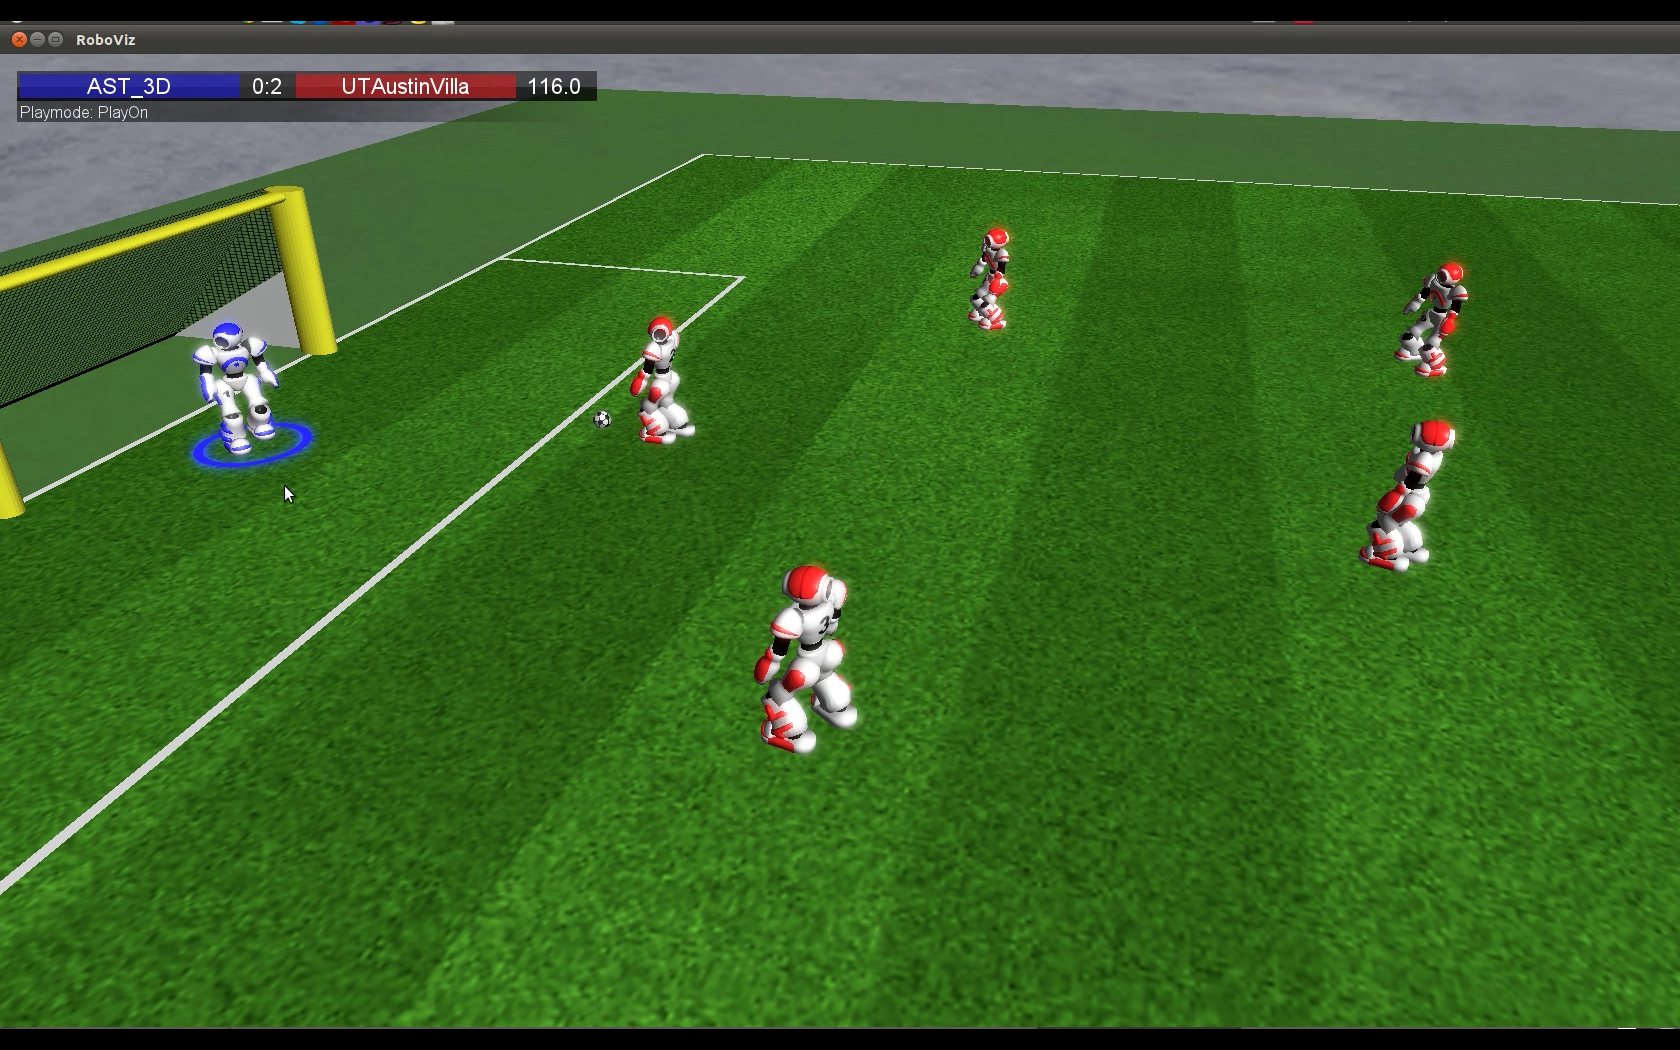
\includegraphics[trim = 5cm 10cm 30cm 5cm, clip,scale=0.25]{Chapter3/figures/GoalieFall.png}
	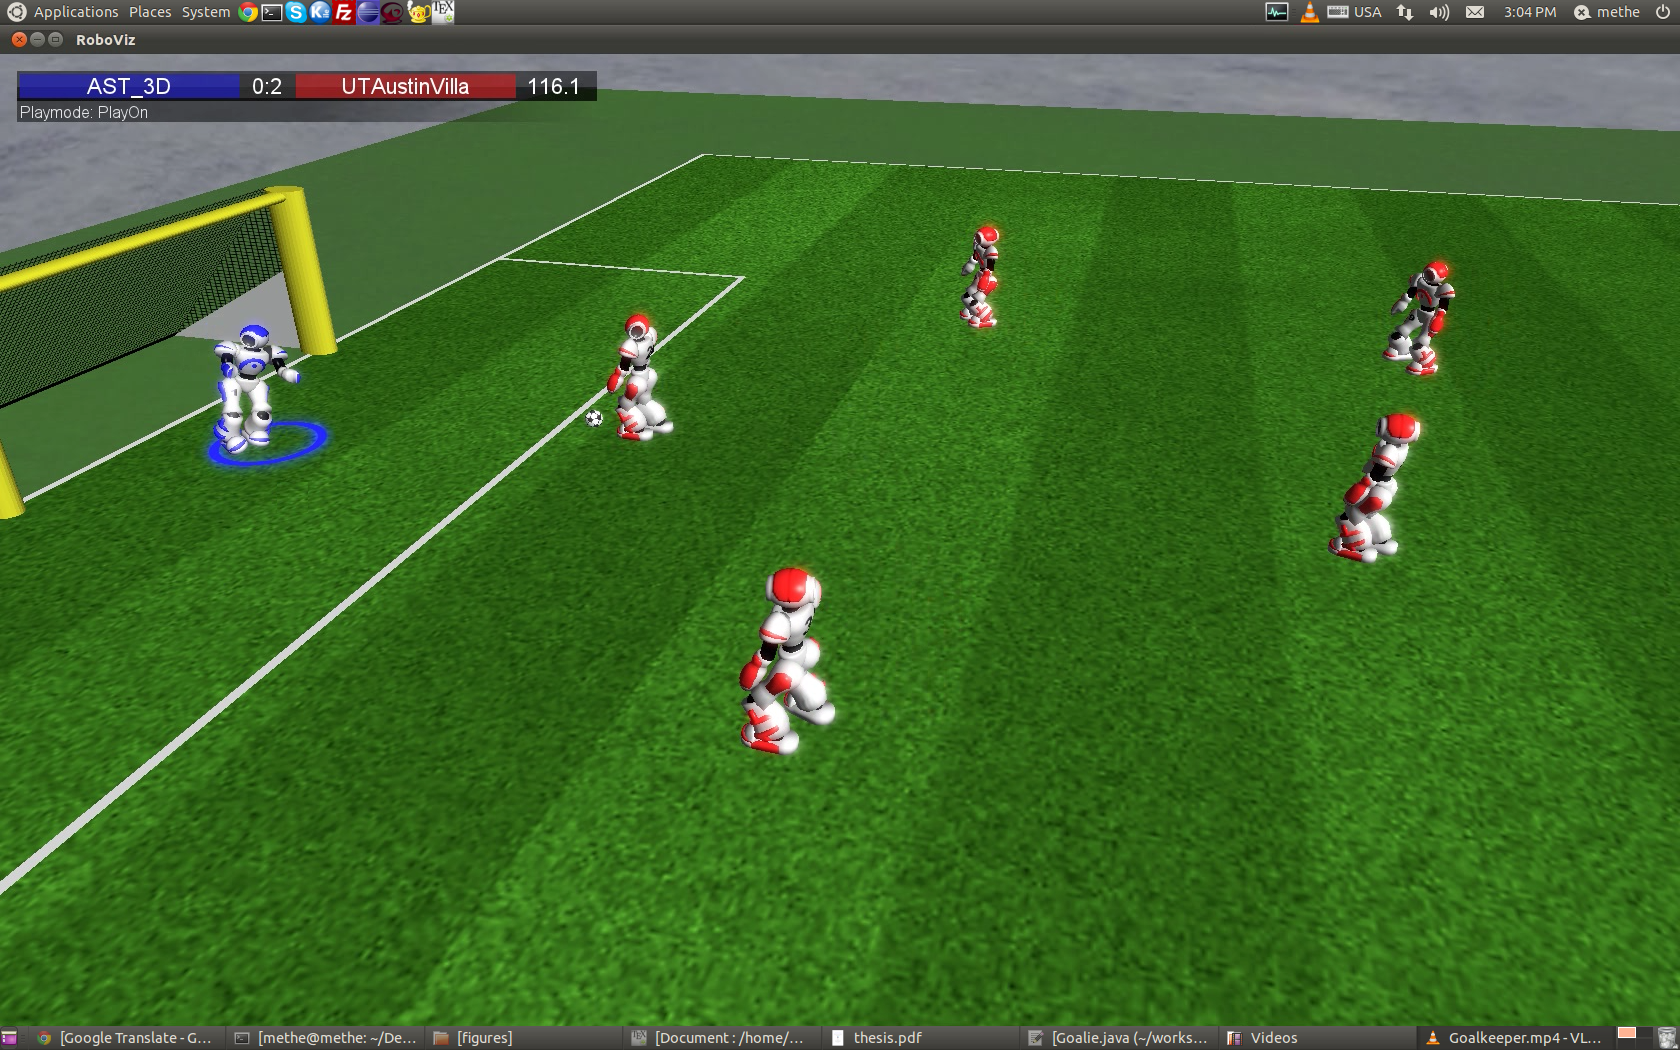
\includegraphics[trim = 5cm 10cm 30cm 5cm, clip,scale=0.25]{Chapter3/figures/GoalieFall2.png}
	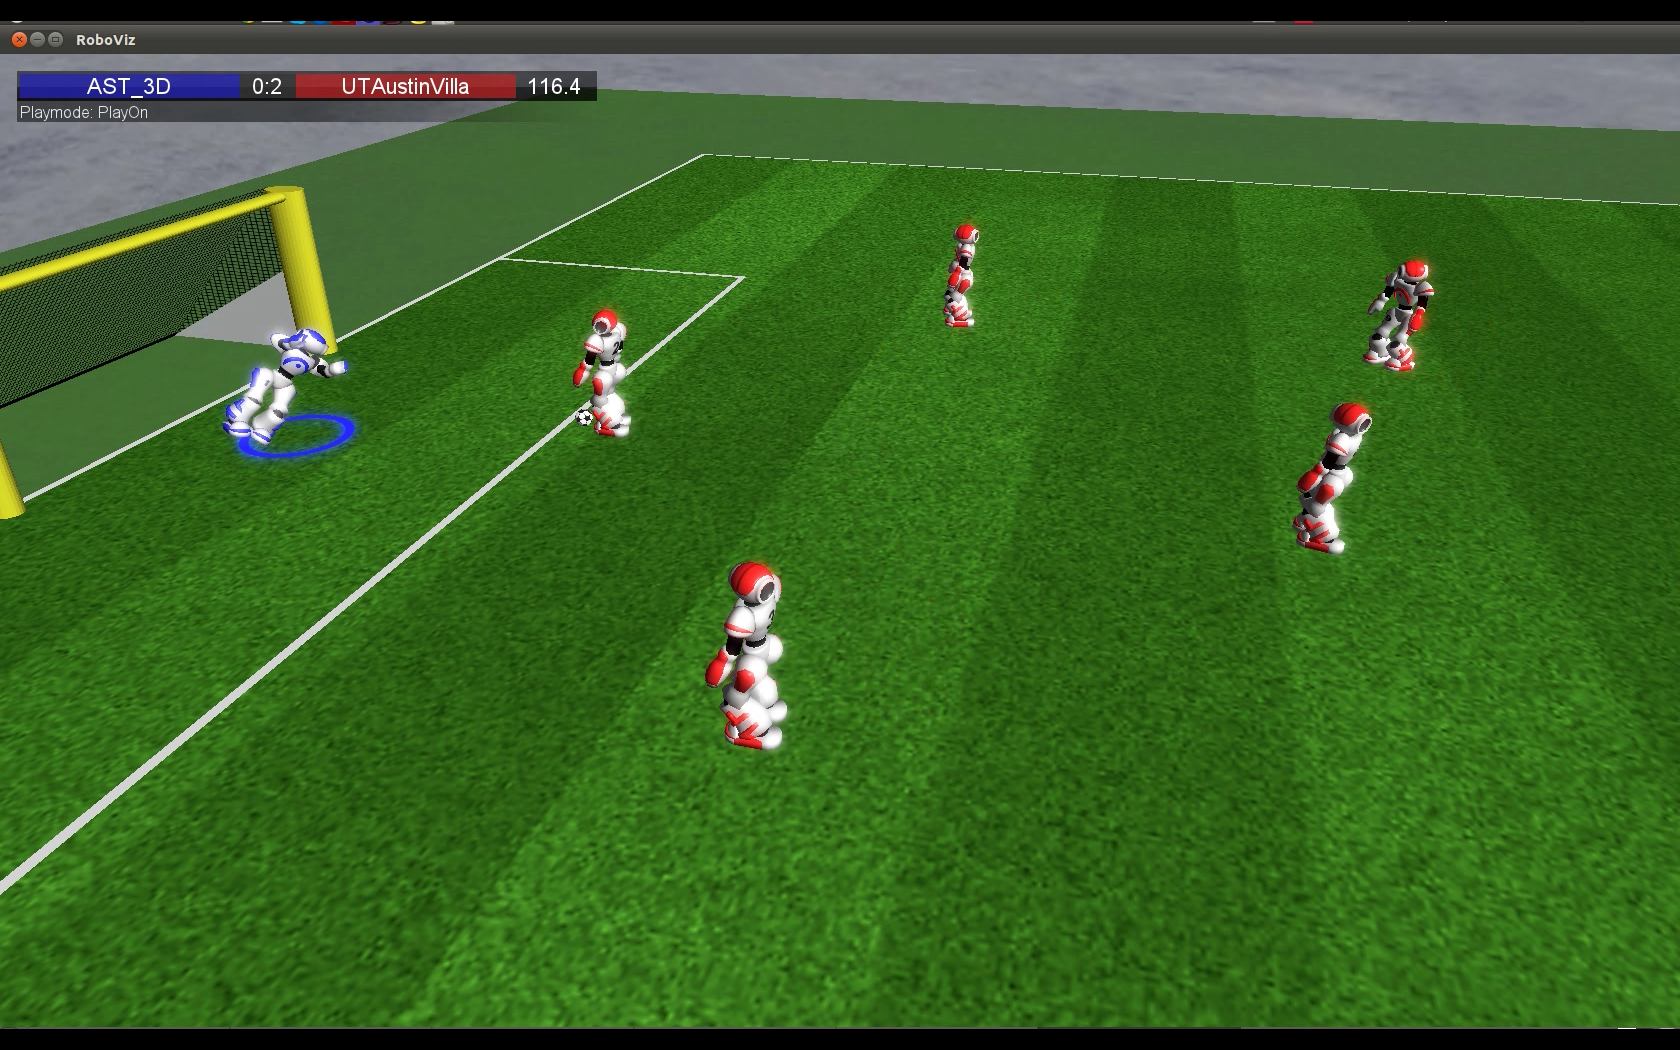
\includegraphics[trim = 5cm 10cm 30cm 5cm, clip,scale=0.25]{Chapter3/figures/GoalieFall3.png}
	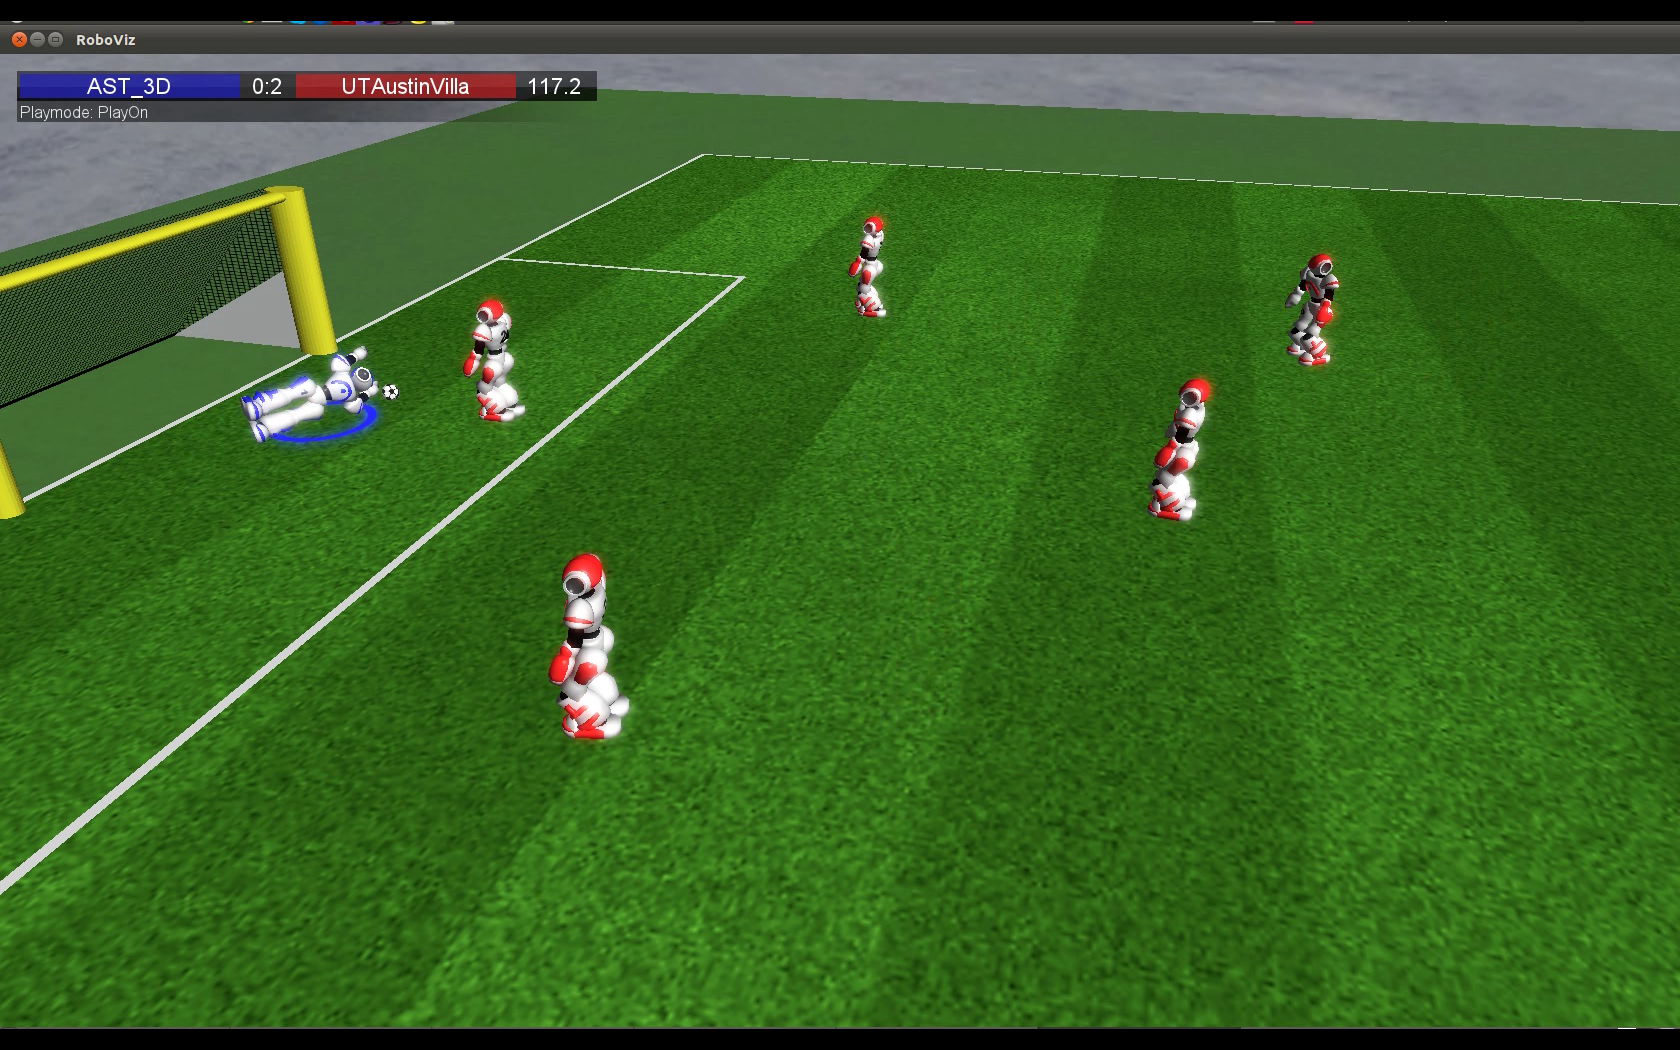
\includegraphics[trim = 5cm 10cm 30cm 5cm, clip,scale=0.25]{Chapter3/figures/GoalieFall4.png}
	\caption{Goalkeeper Falls to Prevent Opponents from Scoring.}
  \label{fig:GoalkeeperFall}
\end{figure}

